\chapter{Software}\label{ch:system-development}
The software is based on a real time operating system (RTOS).
The software is divided into different tasks, which are handled by the RTOS.


\section{File Tree}
The project files are available on GitHub at \url{https://github.com/JensMoeslund/gps-miniprojekt}.
The file tree is shown below, with descriptions of the files and links to the files on GitHub.

\dirtree{%
    .1 gps-miniprojekt/.
    .2 .cargo/.
    .3 \href{https://github.com/JensMoeslund/gps-miniprojekt/blob/master/.cargo/config.toml}{config.toml} $\longrightarrow$
    \begin{minipage}[t]{7cm}
        Configuration file including target and linker settings{.}
    \end{minipage}.
    .2 src/.
    .3 \href{https://github.com/JensMoeslund/gps-miniprojekt/blob/master/src/gnss.rs}{gnss.rs} $\longrightarrow$
    \begin{minipage}[t]{7cm}
        Library for parsing GNSS NMEA data{.}
    \end{minipage}.
    .3 \href{https://github.com/JensMoeslund/gps-miniprojekt/blob/master/src/kalman.rs}{kalman.rs} $\longrightarrow$
    \begin{minipage}[t]{7cm}
        Library for handling the Kalman filter and state estimation{.}
    \end{minipage}..
    .3 \href{https://github.com/JensMoeslund/gps-miniprojekt/blob/master/src/lib.rs}{lib.rs} $\longrightarrow$
    \begin{minipage}[t]{7cm}
        Main library defining project structure{.}
    \end{minipage}.
    .3 \href{https://github.com/JensMoeslund/gps-miniprojekt/blob/master/src/main.rs}{main.rs} $\longrightarrow$
    \begin{minipage}[t]{7cm}
        Main file defining RTOS tasks and initialization{.}
    \end{minipage}..
    .3 \href{https://github.com/JensMoeslund/gps-miniprojekt/blob/master/src/ms5611.rs}{ms5611.rs} $\longrightarrow$
    \begin{minipage}[t]{7cm}
        Library for handling the MS5611 barometer{.}
    \end{minipage}..
    .2 \href{https://github.com/JensMoeslund/gps-miniprojekt/blob/master/Cargo.toml}{Cargo.toml} $\longrightarrow$
    \begin{minipage}[t]{7cm}
        Compilation and dependency configuration file{.}
    \end{minipage}..
    .2 \href{https://github.com/JensMoeslund/gps-miniprojekt/blob/master/memory.x}{memory.x} $\longrightarrow$
    \begin{minipage}[t]{7cm}
        Memory layout file for the microcontroller{.}
    \end{minipage}..
    .2 \href{https://github.com/JensMoeslund/gps-miniprojekt/blob/master/rust-toolchain.toml}{rust-toolchain.toml} $\longrightarrow$
    \begin{minipage}[t]{7cm}
        Rust toolchain configuration file{.}
    \end{minipage}..
}

\section{External dependencies}\label{sec:external-dependencies}
The software uses the following external dependencies:
\begin{itemize}
    \item \textbf{nalgebra} is a linear algebra library for Rust.
    \item \textbf{rtic} is a real-time interrupt-driven concurrency (RTIC) framework for building concurrent applications in Rust.
    \item \textbf{nmea0183} is a library for parsing NMEA 0183 data.
\end{itemize}
\subsection{nalgebra}
The nalgebra library is used for linear algebra operations.%TODO: indsæt kilde
The library is used for matrix operations, such as matrix multiplication, matrix inversion, and matrix addition.

\subsection{RTIC}
The RTOS used in this project is RTIC.%TODO: indsæt kilde til rtic
RTIC is a real-time interrupt-driven concurrency (RTIC) framework for building concurrent applications in Rust.

RTIC is based on the concept of tasks, which are functions that can be executed concurrently.
Tasks can be hardware tasks, which are triggered by interrupts, or software tasks, which are triggered by the RTOS through the use of interrupts.

RTIC also provides a message queue, which can be used to send messages between tasks.
The message queue is a FIFO queue, which can be used to send messages of a fixed size between tasks.

RTIC requires the use of an initialization function, which is used to initialize the hardware and the RTOS.
In the initialization function, the static resources are initialized, and the peripherals are configured.
\subsection{nmea0183}
The nmea0183 library is used for parsing NMEA 0183 data.
The library is used to parse the NMEA data from the GNSS module, and extract the relevant information, such as latitude, longitude, altitude, and speed.%TODO: indsæt kilde

\section{Tasks}
The software is divided into the following tasks:
\begin{itemize}
    \item \textbf{GNSS Sampling Task:} This task is responsible for reading the raw GNSS data and storing it in a buffer.
    \item \textbf{Barometer Sampling Task:} This task is responsible for sampling the barometer, parsing the data and storing it in a buffer.
    \item \textbf{NMEA Parsing Task:} This task is responsible for parsing the NMEA data from the GNSS, and storing the parsed data in a buffer.
    \item \textbf{Kalman Filter Task:} This task is responsible for running the Kalman filter using the data from the GNSS and the barometer.
\end{itemize}
A block diagram of the start of the program is seen in Figure~\ref{fig:initial-block-diagram}.
\begin{figure}[H]
    \centering
    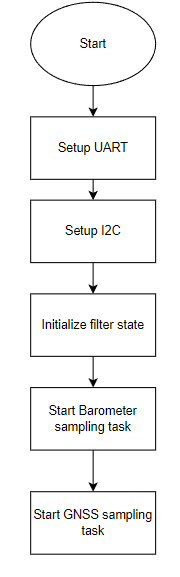
\includegraphics[width=0.3\textwidth]{chapters/04Software/figures/bob}
    \caption{Initial block diagram of the software.}
    \label{fig:initial-block-diagram}
\end{figure}

The init function then starts the tasks.
The flow of the remaining program can be seen in Figure~\ref{fig:flow-diagram}.
\begin{figure}[H]
    \centering
    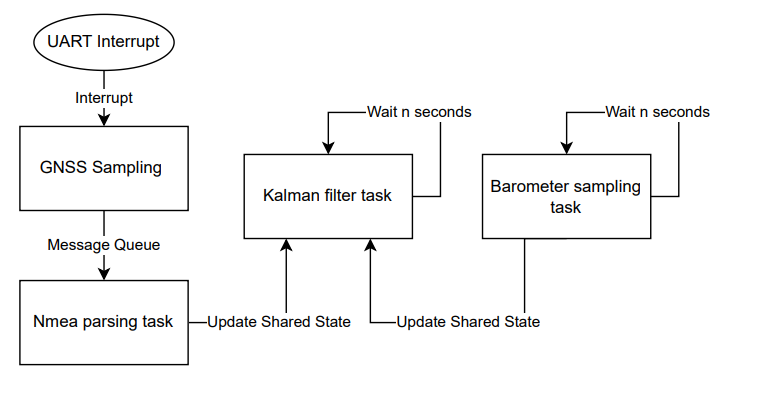
\includegraphics[width=0.8\textwidth]{chapters/04Software/figures/blockdiagram_loop}
    \caption{Flow diagram of the software.}
    \label{fig:flow-diagram}
\end{figure}

The GNSS Sampling Task is responsible for reading the raw GNSS data, but since the data is sent over UART, with a certain time interval, the task must be a hardware task, reacting on the interrupt from the UART.
For every recieved byte, the task will send the byte in a message queue, which the NMEA Parsing Task will read from.

The Barometer Sampling Task is responsible for reading the barometer data.
The sensor is connected to the I2C bus, and will return the data when requested.
For this reason, the task will be a software task, polling the sensor at a certain time interval.

The NMEA Parsing Task is responsible for parsing the NMEA data from the GNSS.
The task will read the data from the message queue, and parse the data.
The parsed data will be stored in a buffer, which the Kalman Filter Task will read from.

The Kalman Filter Task is responsible for running the Kalman filter.
It runs with a certain time interval, and reads the data available in the buffer at that time.


%\chapter{Test}\label{sec:Test}

The Figure~\ref{fig:physical_setup} is made using python and several different libraries.
The output from the python script is a pdf file, which is then included in the document.
\begin{figure}[H]
    \centering
    \includegraphics[width=0.5\textwidth]{02Multipath_illustration_of_multipath}
    \caption{The physical setup of the test}
    \label{fig:physical_setup}
\end{figure}
